% Dataset stats: HMDl-IAI
\begin{figure}[t]
%\captionsetup[subfigure]{labelformat=empty}
\centering
\subfloat[\Gls{teental}]{\label{fig:dstats:HMDl:IAI:teen}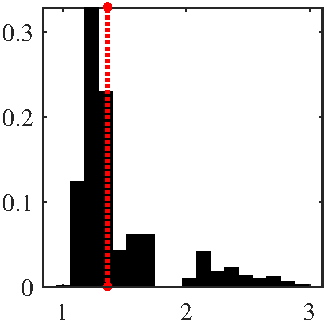
\includegraphics[scale=1]{dstats/HMDl-teen-IAI.pdf}} \hspace{0.5cm} 
\subfloat[\Gls{ektal}]{\label{fig:dstats:HMDl:IAI:ek}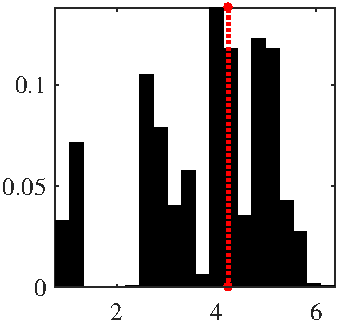
\includegraphics[scale=1]{dstats/HMDl-ek-IAI.pdf}} \\ 
\subfloat[\Gls{jhaptal}]{\label{fig:dstats:HMDl:IAI:jhap}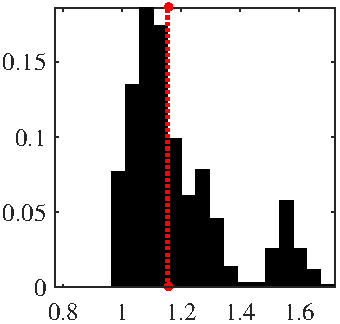
\includegraphics[scale=1]{dstats/HMDl-jhap-IAI.pdf}} \hspace{0.5cm} 
\subfloat[\Gls{rupak}]{\label{fig:dstats:HMDl:IAI:rupak}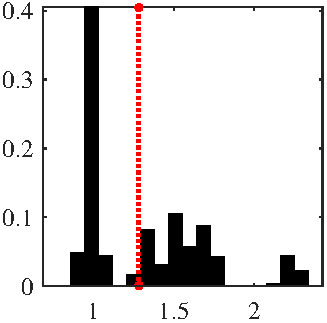
\includegraphics[scale=1]{dstats/HMDl-rupak-IAI.pdf}} \\ 
\caption[HMDl-IAI]{HMDl-IAI}\label{fig:dstats:HMDl:IAI}
\end{figure}
%
%
% Dataset stats: HMDl-IAInorm
\begin{figure}[t]
%\captionsetup[subfigure]{labelformat=empty}
\centering
\subfloat[\Gls{teental}]{\label{fig:dstats:HMDl:IAInorm:teen}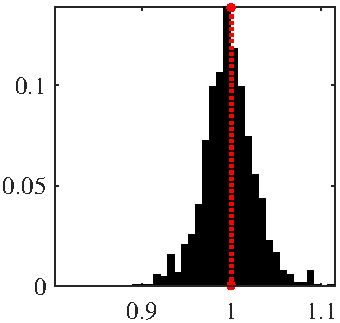
\includegraphics[scale=1]{dstats/HMDl-teen-IAInorm.pdf}} \hspace{0.5cm} 
\subfloat[\Gls{ektal}]{\label{fig:dstats:HMDl:IAInorm:ek}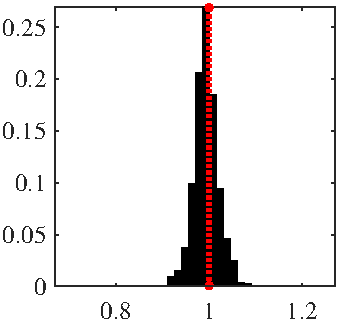
\includegraphics[scale=1]{dstats/HMDl-ek-IAInorm.pdf}} \\ 
\subfloat[\Gls{jhaptal}]{\label{fig:dstats:HMDl:IAInorm:jhap}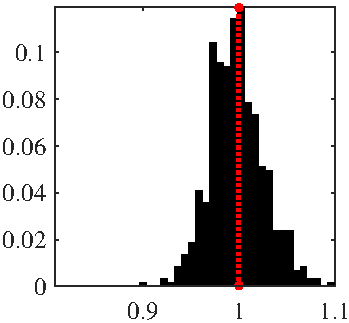
\includegraphics[scale=1]{dstats/HMDl-jhap-IAInorm.pdf}} \hspace{0.5cm} 
\subfloat[\Gls{rupak}]{\label{fig:dstats:HMDl:IAInorm:rupak}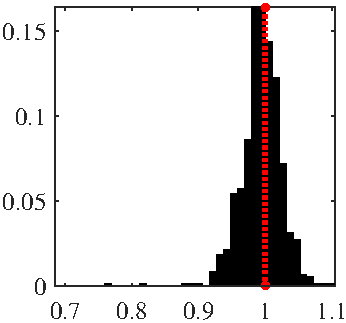
\includegraphics[scale=1]{dstats/HMDl-rupak-IAInorm.pdf}} \\ 
\caption[HMDl-IAInorm]{HMDl-IAInorm}\label{fig:dstats:HMDl:IAInorm}
\centering
\end{figure}
%
%
% Dataset stats: HMDl-ISI
\begin{figure}[t]
%\captionsetup[subfigure]{labelformat=empty}
\centering
\subfloat[\Gls{teental}]{\label{fig:dstats:HMDl:ISI:teen}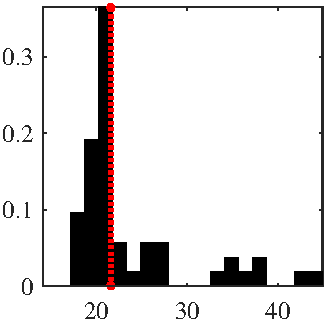
\includegraphics[scale=1]{dstats/HMDl-teen-ISI.pdf}} \hspace{0.5cm} 
\subfloat[\Gls{ektal}]{\label{fig:dstats:HMDl:ISI:ek}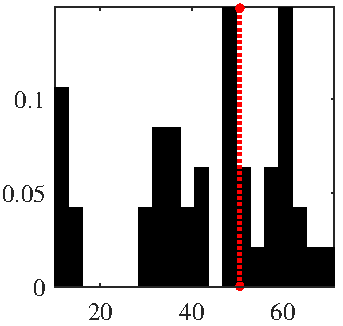
\includegraphics[scale=1]{dstats/HMDl-ek-ISI.pdf}} \\ 
\subfloat[\Gls{jhaptal}]{\label{fig:dstats:HMDl:ISI:jhap}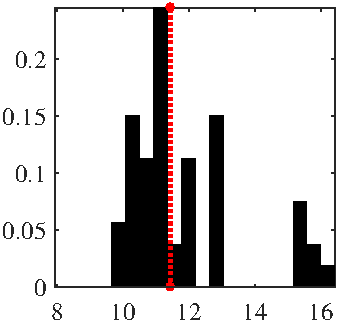
\includegraphics[scale=1]{dstats/HMDl-jhap-ISI.pdf}} \hspace{0.5cm} 
\subfloat[\Gls{rupak}]{\label{fig:dstats:HMDl:ISI:rupak}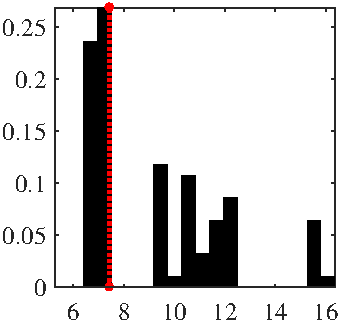
\includegraphics[scale=1]{dstats/HMDl-rupak-ISI.pdf}} \\ 
\caption[HMDl-ISI]{HMDl-ISI}\label{fig:dstats:HMDl:ISI}
\end{figure}
%
%
% Dataset stats: HMDl-ISInorm
\begin{figure}[t]
%\captionsetup[subfigure]{labelformat=empty}
\centering
\subfloat[\Gls{teental}]{\label{fig:dstats:HMDl:ISInorm:teen}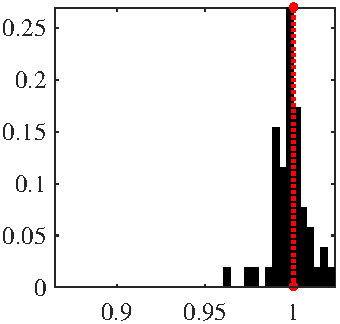
\includegraphics[scale=1]{dstats/HMDl-teen-ISInorm.pdf}} \hspace{0.5cm} 
\subfloat[\Gls{ektal}]{\label{fig:dstats:HMDl:ISInorm:ek}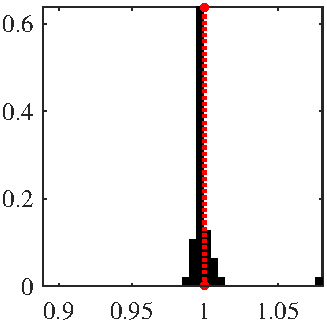
\includegraphics[scale=1]{dstats/HMDl-ek-ISInorm.pdf}} \\ 
\subfloat[\Gls{jhaptal}]{\label{fig:dstats:HMDl:ISInorm:jhap}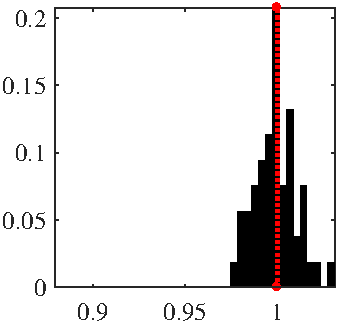
\includegraphics[scale=1]{dstats/HMDl-jhap-ISInorm.pdf}} \hspace{0.5cm} 
\subfloat[\Gls{rupak}]{\label{fig:dstats:HMDl:ISInorm:rupak}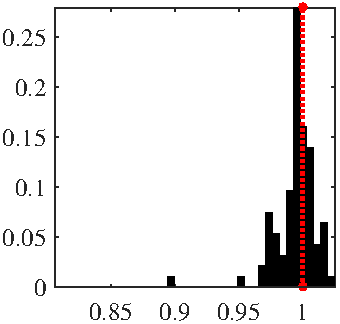
\includegraphics[scale=1]{dstats/HMDl-rupak-ISInorm.pdf}} \\ 
\caption[HMDl-ISInorm]{HMDl-ISInorm}\label{fig:dstats:HMDl:ISInorm}
\end{figure}
%
%